\documentclass[border=10pt]{standalone}

\usepackage{tikz}
\usepackage{tikzsymbols}
\usetikzlibrary{calc,patterns,shapes.geometric}

\def\centerarc[#1](#2)(#3:#4:#5){\draw[#1] ($(#2)+({#5*cos(#3)},{#5*sin(#3)})$) arc (#3:#4:#5);}

\begin{document}
	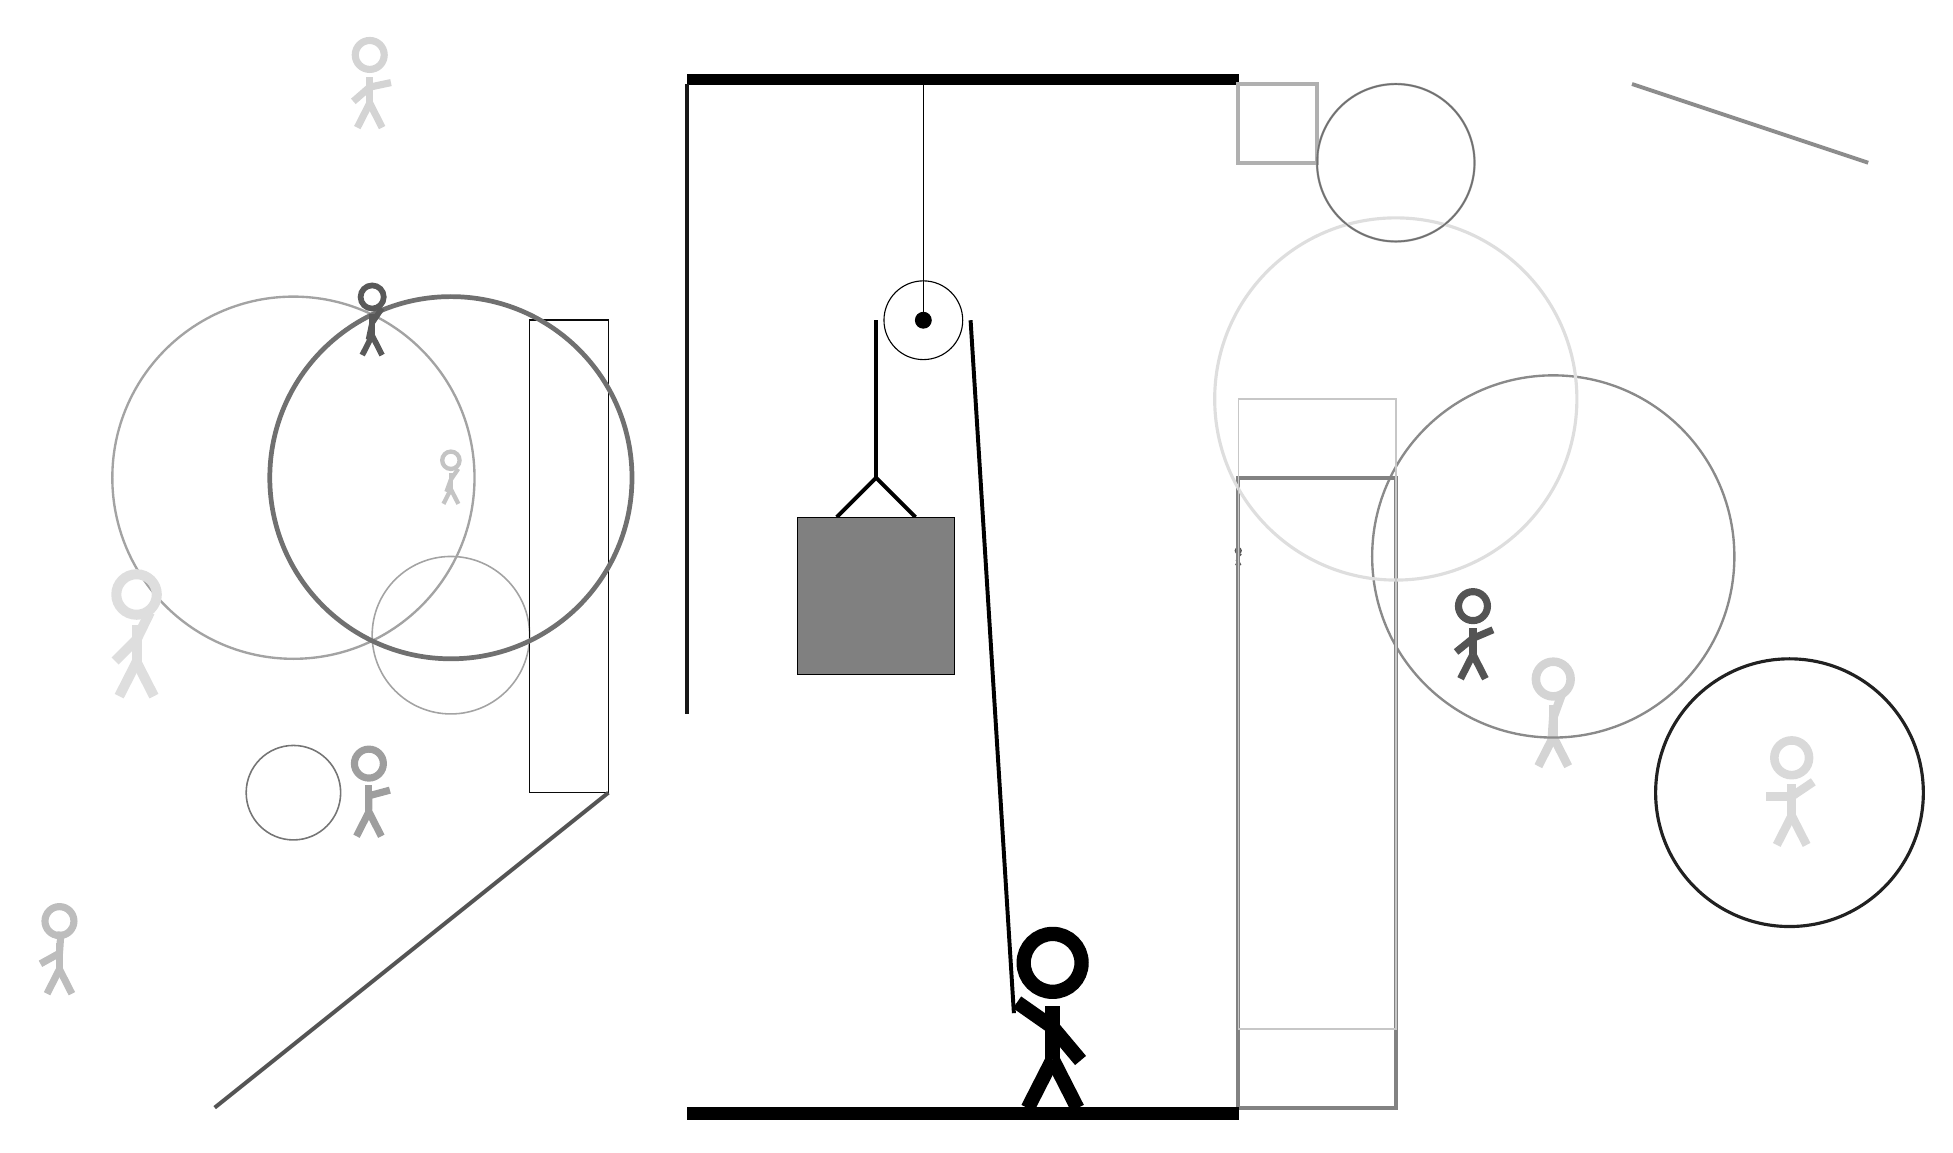
\begin{tikzpicture}
		%%%%% START %%%%%
		
		\draw[fill=black] (-2, 10) rectangle (5, 10.125);
		
		\draw (1, 7) circle (0.5);
		\draw[fill=black] (1, 7) circle (0.1);
		\draw (1, 10) -- (1, 7);
		
		\draw[line width=0.5mm] (-0.1, 4.5) -- (0.4, 5.0) -- (0.9, 4.5);
		\draw[fill=black!50] (-0.6, 4.5) rectangle (1.4, 2.5);
		
		\node[line width=0.3mm, color=black!17] at (9, 2) {\Strichmaxerl[6][86][70]};
		
		\node[line width=0.7mm, color=black!17] at (-6, 10) {\Strichmaxerl[5][41][12]};
		\node[line width=0.5mm, color=black!66] at (5, 4) {\Strichmaxerl[1][63][46]};
		\draw [line width=0.3mm, color=black!46](9, 4) circle (2.3);
		\draw[line width=0.5mm, color=black!49] (7, 5) rectangle (5, -3);
		\node[line width=0.3mm, color=black!15] at (12, 1) {\Strichmaxerl[6][0][34]};
		\draw[line width=0.5mm, color=black!45](10, 10) -- (13, 9);
		\draw [line width=0.4mm, color=black!87](12, 1) circle (1.7);
		\draw [line width=0.3mm, color=black!31](7, 9) circle (1.0);
		\draw[line width=0.5mm, color=black!31] (5, 10) rectangle (6, 9);
		\draw[line width=0.5mm, color=black!91] (-2, 2) rectangle (-2, 10);
		\draw [line width=0.6mm, color=black!28](-5, 5) circle (0.0);
		\draw [line width=0.4mm, color=black!13](7, 6) circle (2.3);
		
		\draw [line width=0.2mm, color=black!36](-5, 3) circle (1.0);
		\draw[line width=0.2mm, color=black!96] (-3, 7) rectangle (-4, 1);
		\node[line width=0.5mm, color=black!26] at (-10, -1) {\Strichmaxerl[5][29][86]};
		
		\draw [line width=0.2mm, color=black!54](-7, 1) circle (0.6);
		\draw [line width=0.3mm, color=black!36](-7, 5) circle (2.3);
		\node[line width=0.6mm, color=black!38] at (-6, 1) {\Strichmaxerl[5][89][15]};
		\draw[line width=0.2mm, color=black!22] (5, 6) rectangle (7, -2);
		\draw [line width=0.2mm, color=black!56](7, 9) circle (1.0);
		\draw[line width=0.5mm, color=black!67](-3, 1) -- (-8, -3);
		\draw [line width=0.6mm, color=black!56](-5, 5) circle (2.3);
		\node[line width=0.2mm, color=black!13] at (-9, 3) {\Strichmaxerl[7][45][64]};
		\node[line width=0.7mm, color=black!67] at (8, 3) {\Strichmaxerl[5][39][23]};
		
		\node[line width=0.4mm, color=black!23] at (-5, 5) {\Strichmaxerl[3][70][56]};
		\node[line width=0.2mm, color=black!65] at (-6, 7) {\Strichmaxerl[4][78][56]};
		
		\draw[line width=0.5mm] (0.4, 7) -- (0.4, 5.0);
		\centerarc[line width=0.5mm](1, 7)(0:180:0.6);
		\draw[line width=0.5mm](1.6, 7) -- (2.15, -1.8);
		
		\node at (2.6, -1.9) {\Strichmaxerl[10][-35][-50]};
		
		\draw[fill=black] (-2, -3) rectangle (5, -3.15);
		
		%%%%% END %%%%%
	\end{tikzpicture}
\end{document}